\section{Stationäre Strömungsanalyse (SCD, Stationray Current Distribution)}
Die stationäre Strömungsanalyse wird für die Berechnung des Ersatzwiderstand gebraucht
\subsection{Integralgleichungen}
\begin{tabular}{|p{.30\textwidth} |p{.70\textwidth}|}
	\hline 
	\textbf{Elektrische Stromdichte} \newline
	\tabbild[width=3cm]{images/ElStromdichte} & Die elektrische Stromdichte kennzeichnet wie dicht zusammengedrängt ein elektrischer Strom fliesst. Damit ist auch die Belastung eines Leiters durch den Strom bekannt.\newline
	\[ \vec{J} = \dfrac{dI}{dA}\cdot \vec{n}\qquad [\vec{J}] = \dfrac{A}{m^2} \] \[I = \iint\limits_{(A)}\vec{J}\cdot\vec{dA} \] \\
	\hline
	\textbf{Kontinuitätsgleichung} \newline
	\tabbild[width=3cm]{images/Gauss.png} & Der herausfliessende Strom aus einer geschlossenen Fläche ist gleich der Abnahme der Ladung \newline
		\[ I = -\dfrac{dQ}{dt} = -\dfrac{d}{dt}\iiint\limits_{(V)}\varrho\cdot dV = -\iiint\limits_{(V)}\dfrac{d\varrho}{dt}\cdot dV \]
	 \[ \varoiint\limits_{(A)}\vec{J}\cdot\vec{dA} = -\iiint\limits_{(V)}\dfrac{d\varrho}{dt}\cdot dV \]
	\[ \varoiint\limits_{(A)}\vec{J}\cdot\vec{dA} = 0\] \\
	\hline
	\textbf{Ohmsches Gesetz}\newline
	\tabbild[width=3cm]{images/OhmschesGesetz.png} & 
	\[ J= \sigma \cdot E\]
	\[ R = \varrho\cdot\dfrac{l}{A}\]
	\[ \sigma = \dfrac{1}{\varrho}\]
	\[ G = \sigma\cdot\dfrac{A}{l} \]\\
	\hline
\end{tabular}
\subsection{Differenzialgleichungen der elektrostatischen Analyse}
\begin{multicols}{2}
	\textbf{Stationäre Analyse}\\
	\[\nabla \vec{J} = -\frac{d \rho}{dt}=0\]
	\textbf{Laplace Gleichung}
	\[\dfrac{\partial^2\varphi}{\partial x^2} +  \dfrac{\partial^2\varphi}{\partial y^2} + \dfrac{\partial^2\varphi}{\partial z^2} = \Delta \varphi = 0\]	
\end{multicols}
\clearpage
\pagebreak
\subsection{Randbedingungen}
\begin{minipage}{8cm}
	\begin{itemize}
		\item Der geerdete Rand \[\varphi = 0\]
		\item Der Rand mit bekannten Potential \[ \varphi = U \]
		\item Der Rand der Symmetrie \[ \dfrac{\partial\varphi}{\partial n} = 0\]
		\item Der Rand zwischen zwei Materialien \[\sigma_{1} \cdot \frac{d \varphi_{2}}{dn}=\sigma_{2} \cdot \frac{d \varphi_{1}}{dn}\]
	\end{itemize}
\end{minipage}
\begin{minipage}{8cm}
	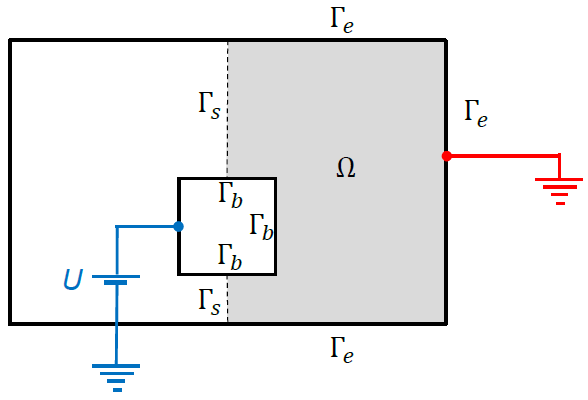
\includegraphics[width=8cm]{images/randbedinung_ES.png}
\end{minipage}
\subsection{Anwendung}
%TODO Beispiel einfügen
\clearpage
\pagebreak